\documentclass{article}
\usepackage[preprint]{neurips_2019}
\usepackage{graphicx,float}
% \usepackage[utf8]{inputenc} % allow utf-8 input
% \usepackage[T1]{fontenc}    % use 8-bit T1 fonts
% \usepackage{hyperref}       % hyperlinks
% \usepackage{url}            % simple URL typesetting
% \usepackage{booktabs}       % professional-quality tables
% \usepackage{amsfonts}       % blackboard math symbols
% \usepackage{nicefrac}       % compact symbols for 1/2, etc.
% \usepackage{microtype}      % microtypography
\title{Predicting Stocks Trends Based on News}
\author{
Harsh Dedhiya, Raghav Malhotra, Phumin Walaipatchara\\
Department of Computer Science\\
Boston University\\
\texttt{hdedhiya@bu.edu, raghav20@bu.edu, phuminw@bu.edu}\\
}
\begin{document}
\maketitle
\begin{abstract}
    To add abstract bibibikb
\end{abstract}
\section{Background}
Stocks market has been known to be volatile and sentitive to facctors, including news and statistics.
 Speculation on stocks movement requires complicated techniques and models, still the result is not
 satisfactory.
\subsection{Indicators}
Nothing here for now 

\section{Dataset}
Some text for second section

\section{Na\"ive Bayes}
Describe the result from Na\"ive Bayes approach

\section{Logistic Regression}
Describe the result from logictic regression

\section{Sentiment Analysis}

\section{Recurrent Neural Network}
\indent In order to capture the objective of accurate prediction, Recurrent Neural Network (RNN) is introduced
 because its ability to exhibit internal state (memory). Specifically, Long short-term memory (LSTM),
 a special kind of RNN, is used for implementation as LSTM can deal with vanishing gradient problems
 and is capable of learning long-term dependencies.
\\
\begin{figure}
    \centering
    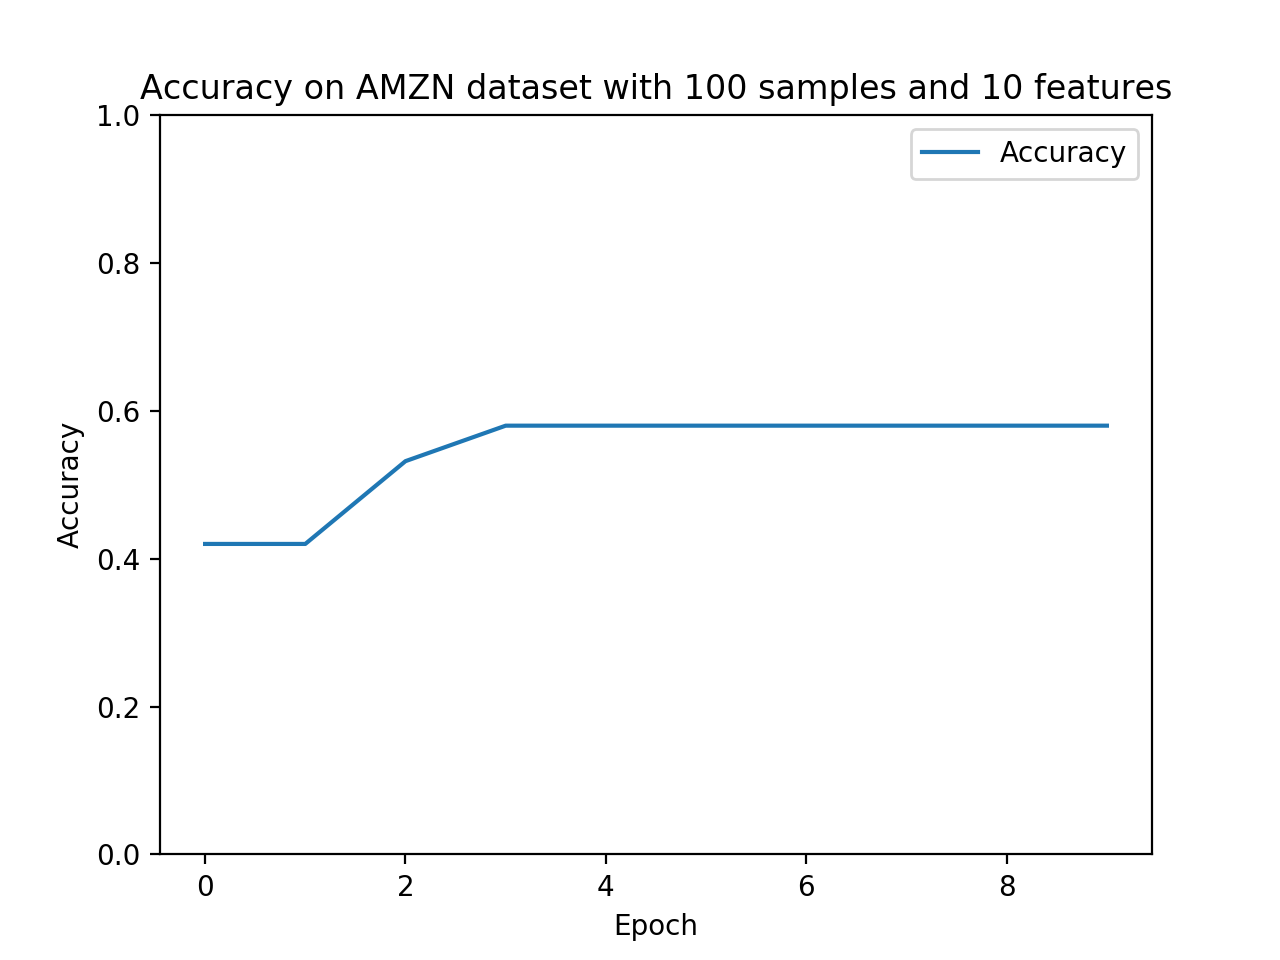
\includegraphics[scale=0.5]{assets/Accuracy.png}
    \caption{Accuracy of the model}
\end{figure}
Before begin training the model, the dataset, 100 samples in this case, must be preprocesed introduced
 boolean vector through $TfidfVectorizer$ from $sklearn.feature\_extraction.text$. The $max_features$, which is
 also the size of the boolean vector is specified to be 10. Each sample (now a boolean vector) is paired up with
 the stock (AMZN in this case) movement, 1 for going up and 0 otherwise. In one epoch, we use $KFold$ from
 $sklearn.model_selection$ to split the dataset into 2 groups, one for training and one for testing.
\\\\
 Regarding network structure, the LSTM network has 10 input nodes, which corresponds to the size of
 the boolean vector. It has 4 hidden nodes between the input layer and the LSTM and use sigmoid as an activation
 function. After LSTM module, the output layer consisting of 2 nodes uses softmax as an activation function in order
 to represent output as a probability of classification.
\section*{References}
if needed

\end{document}
